\section{Auswertung}
\label{sec:Auswertung}

\subsection{Impulshöhen}

Die gemessenen Impulssignale mit und ohne Verstärker werden in Abbildung \ref{fig:mit} und \ref{fig:ohne} dargestellt.

\begin{figure}[H]
  \centering
  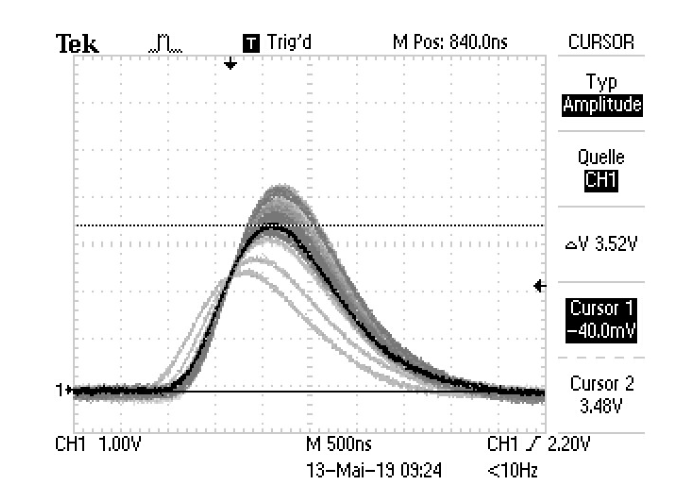
\includegraphics[height=8cm]{mitverstaerker.png}
  \caption{Impulshöhen mit Verstärker}
  \label{fig:mit}
\end{figure}

\begin{figure}[H]
  \centering
  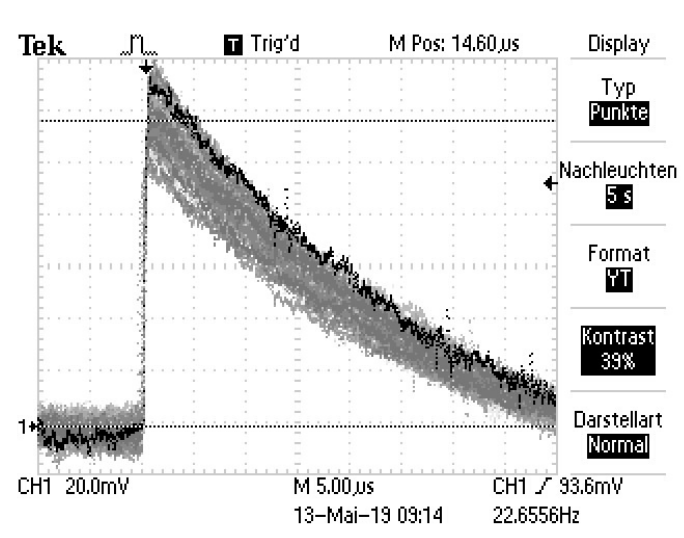
\includegraphics[height=8cm]{ohneverstaerker.png}
  \caption{Impulshöhen ohne Verstärker}
  \label{fig:ohne}
\end{figure}

Die Anstiegszeit des Signals mit Verstärker beträgt $\SI{1.3}{\micro\second}$ und die ohne Verstärker $\SI{1}{\micro\second}$.




\subsection{Bestimmung der Foliendicke}
In Tabelle 1 sind die gemessenen Spannungen in Abhängigkeit des Kammerderuckes mit und ohne Goldfolie dargesellt.

\begin{table}[H]
\centering
\caption{Spannungen in Abhängigkeit des Kammerdruckes }
\sisetup{table-format=2.1}
\begin{tabular}{S S S| S S S}
  \toprule
    \multicolumn{3}{c}{Ohne Folie} & \multicolumn{3}{c}{Mit Folie} \\
    \cmidrule(lr){1-3}\cmidrule(lr){4-6}
    {$p/$mbar} & {$U/\, \symup{V}$} & {Fehler/V} & {$p$/mbar} & {$U/\, \symup{V}$} & {Fehler/V} \\
    \midrule
    0.09  & 3.66 &  0.5 & 0.12 & 2.66 & 0.5 \\
    10.0   & 3.64 &  0.5 & 10.7 & 2.50 & 0.6 \\
    20.0   & 3.52 &  0.5 & 20.5 & 2.40 & 0.6 \\
    29.8   & 3.32 &  0.5 & 32.3 & 2.30 & 0.6 \\
    40.1   & 3.32 &  0.5 & 40.8 & 2.16 & 0.6 \\
    50.2   & 3.20 &  0.6 & 50.7 & 2.00 & 0.7 \\
    60.1   & 3.12 &  0.6 & 61.2 & 1.88 & 0.6 \\
    70.5   & 3.00 &  0.5 & 72.0 & 1.74 & 0.6 \\
    80.2   & 2.96 &  0.4 & 82.3 & 1.70 & 0.7 \\
    91.8   & 2.88 &  0.5 & 92.2 & 1.58 & 0.7 \\
    100.2  & 2.80 &  0.5 & 100.7& 1.50 & 0.7 \\
    111.2  & 2.70 &  0.4 & 111.0& 1.38 & 0.8 \\
    121.2  & 2.30 &  0.5 & 122.0& 1.16 & 0.5 \\
    132.2  & 2.20 &  0.5 & 131.3& 1.04 & 0.5 \\
    141.7  & 2.10 &  0.5 & 142.9& 0.91 & 0.5 \\
    151.1  & 2.00 &  0.5 & 150.7& 0.76 & 0.3 \\
    162.2  & 1.70 &  0.5 & 160.9& 0.72 & 0.3 \\
    171.2  & 1.64 &  0.5 & 172.7& 0.68 & 0.3 \\
    181.3  & 1.58 &  0.6 & 198.0& 0.40 & 0.2 \\
    190.5  & 1.50 &  0.5 & & & \\
    200.8  & 1.30 &  0.5 & & & \\
    217.6  & 1.00 &  0.6 & & & \\
      \bottomrule
  \end{tabular}
\end{table}





\subsection{Differentieller Wirkungsquerschnitt}
In Tabelle 2 wird die Zählrate $N$ in Abhängigkeit des Winkels $\Theta$ und der Messzeit $t$ dargestellt.


\begin{table}[H]
  \centering
  \caption{Zählrate in Abhängigkeit von Winkel und Messzeit}
  \label{tab:Parameter}
  \begin{tabular}{c c c}
    \toprule
    N & $\Theta/$° & $t$ /s\\
    \midrule
    2219 &  0 & 200 \\
    2120 &  1 & 200 \\
    1748 &  2 & 200 \\
    1477 &  3 & 200 \\
    1684 &  4 & 300 \\
    1317 &  5 & 300 \\
    1218 &  6 & 400 \\
    1199 &  7 & 600 \\
     764 &  8 & 600 \\
     519 & 10 & 600 \\
     231 & 12 & 600 \\
      83 & 15 & 600 \\
      34 & 18 & 600 \\
      25 & 20 & 600 \\
    \bottomrule
  \end{tabular}
\end{table}

Der differentielle Wirkungsquerschnitt wird nun aus der Gleichung
\begin{equation}
  \frac{\symup{d}\sigma}{\symup{d}\Omega} = \frac{N}{t \cdot I_0 \cdot N_\symup{Au} \cdot \Delta x \cdot \Delta \Omega}
  \label{eqn:wq}
\end{equation}
berechnet.

Dabei ist $I_0$ die Zählrate der Nullmessung ohne Folie und ergibt sich zu $I_0 =\SI{20.83(26)}{1\per\second}$.

$\Delta \Omega$ bezeichnet den pyramidenartigen Raumwinkel, der von
der effektiven Detektorfläche eingenommen wird. Um diesen zu berechnen, muss
als erstes die effektive Detektorfläche selbst bestimmt werden. Dies geschieht
mithilfe der Abbildung \ref{fig:aufbau}. Die gesuchte Breite $b$ und Höhe $h$ der
besagten Fläche lassen sich berechnen aus

\begin{align*}
  b &= \frac{b_\symup{b} \cdot d}{c} \\
  h &= \frac{h_\symup{b} \cdot d}{c}
\end{align*}

Dabei bezeichnen $b_\symup{b}$ und $h_\symup{b}$ die Breite und Höhe der Blende.
$c$ ist der Abstand von der Folie zur Blende und $d$ ist der Abstand von der Folie
zur eigentlichen Detektoroberfläche. Es gilt \cite{sample1}:

\begin{align*}
  b_\symup{b} = \SI{2}{\milli\meter} \\
  h_\symup{b} = \SI{10}{\milli\meter} \\
  c = \SI{41}{\milli\meter} \\
  d = \SI{41}{\milli\meter}
\end{align*}
Und daraus ergibt sich
\begin{align*}
  b &= \SI{2.195}{\milli\meter} \\
  h &= \SI{10.976}{\milli\meter}
\end{align*}

Der Raumwinkel ergibt sich dann aus (Quelle)
\begin{equation}
  \Delta \Omega = 4 \cdot \arctan\left(\frac{b \cdot h}{2d \cdot \sqrt{4d^2 + b^2 + h^2}}\right) = \SI{0.0118}{}
\end{equation}

$\Delta x = 2 \cdot 10^{-6} \, \symup{m}$ ist die Dicke der Folie und $N_\symup{Au} = 5,895 \cdot 10^{28} \, 1/\symup{m^3}$ die Atomdichte von Gold. Daraus können dann differentiellen Wirkungsquerschnitte berechnet werden. Die Ergebnisse sind in Tabelle (...) in Abhängigkeit vom Winkel $\Theta$ dargestellt.

Die berechneten Werte und die Theoriekurve, welche sich aus Gleichung \ref{eqn:rutherford} ergibt, werden in Abbilung \ref{fig:wirkungsquerschnitt} dargestellt.

\begin{figure}[H]
  \centering
  \includegraphics{build/winkel.pdf}
  \caption{Berechneter und gemessener differentieller Wirkungsquerschnitt.}
  \label{fig:wirkungsquerschnitt}
\end{figure}
